\documentclass{article}
\usepackage[english]{babel}
\usepackage[utf8]{inputenc}
\usepackage{fancyhdr}
\usepackage[square]{natbib}
\usepackage{multibib}
\newcites{main}{Primary References}
\bibliographystyle{apalike}
\bibliographystylemain{apalike}
\newcites{code}{Code References}
\bibliographystylecode{apalike}
\newcites{soft}{Software References}
\bibliographystylesoft{apalike}
\usepackage{graphicx}
\graphicspath{ {./Images/} }
\usepackage{wrapfig}
\setlength{\abovecaptionskip}{7pt plus 3pt minus 2pt}
\usepackage{geometry}
\geometry{a4paper,left=30mm,top=30mm}
\usepackage{float}
\usepackage{hyperref}

%Titlepage
\thispagestyle{fancy}
\fancyhf{}
\setlength{\headheight}{22.54448pt}
\rhead{University of Sussex - Informatics\\
Computer Science with Artificial Intelligence}
\lhead{Jacob Brown}
\rfoot{
Submission Year - 2022\\
Candidate Number - 198732\\
Project Supervisor - Simon Bowes\\
}

\begin{document}
\paragraph*{
\\
}
\part*{
\begin{center}
{ \Huge ``Lizardbot"}
\\[1\baselineskip]
{\Large A reptile-inspired model of robots optimised to navigate rough terrain}
\end{center}
}
\paragraph*{Abstract\\}
Insert abstract here
%TODO ADD abstract\\
\vspace*{\fill}
\newpage
\pagestyle{fancy}
\fancyhf{}
\rhead{PAGE \thepage}
\lhead{LIZARDBOT - \leftmark}

\tableofcontents

%Report
\newpage
\section{Introduction}
Nature can often inspire elegant and efficient solutions to non-natural problems. The tunnel-building behaviours of ants can be used to generate algorithms to manage traffic flow in a city for example. This can be much more efficient than deploying a group of developers to design an elaborate network to structure how the population navigates the city. Alternatively, the nests of ants could be studied and their tunnel-building algorithm applied to the problem. \citepmain{antCars} \\
In this project, the characteristics of various reptiles will be applied to a model of a robot - “Lizardbot” - to optimise the physical design and algorithm it uses to navigate rough terrain. For robots used in applications such as bomb disposal or interplanetary exploration, the environments that they face can be highly unpredictable. The margin for error is often low to nonexistent, as there can be little physical access to the robot to fix any issues. These robots require a design and an algorithm optimised to enable them to traverse any landscape they are presented with. \\

On a climbing trip to the Isle of Portland I took a break from repeatedly falling off the cliff to watch a lizard. It was attempting to jump from the path onto a nearby rock. Every time it failed it paused, then tried again with its tail in a completely different position. It was naturally using its tail to counterbalance its body as it jumped, and learning from previous attempts. The addition of a tail to a robot can produce an efficient jumping robot with the application of relatively simple maths. A prime example of this is shown in the \textit{‘UC Berkeley Leaping Lizard \& Robot}’ video.\\ \citepmain{agamaVideo} This behaviour can be observed elsewhere in nature; when a praying mantis jumps it swings its body and abdomen to ensure it hits its target, \citepmain{prayingMantis}  or when cats twist their bodies to reorient themselves to land on their feet. \citepmain{catsLanding}
The lizard’s stabilising tail, alongside other reptilian characteristics, could provide a nature-inspired solution for a robot targeting rough terrain. Since I lack the resources required to test this by building a physical robot, the popular gaming engine Unity \citepsoft{unity} will be used to create a virtual model of the robot instead. The Unity engine has built-in physics, collision, and terrain features that bring complex interactions within scope.


\newpage
\section{Project Aims}
The project can be divided into three areas: the structure of the model, the movement algorithm, and the generation of the terrain. \\

%TODO ADD explanation of why the robot is being modelled instead of physically built\\

%TODO ADD explanation of why Unity was chosen
\subsection{Primary Objectives}
\subsubsection{Robot Design}
This project will focus on determining how various reptilian characteristics influence the success of the model as it navigates an example terrain. The objective is to explore the ‘ideal’ design of a robot, and the relationship between this body and its navigation of a randomly generated terrain. The basic performance metric will be how far it successfully moves across the terrain (in a straight line from the origin) before it gets stuck. This final state may be bouncing back and forth between two points or hitting a section of the terrain that it cannot progress past; the algorithm to determine if the robot is trapped will consider both of these possibilities. \\
Within this bigger picture goal there will be several smaller experiments into how various features / approaches influence the outcome. \\

The body of the robot will emulate that of a snake such that it will be constructed of a series of independent modules / sections located linearly behind the head. This design \textit{"provides the ability of traversing in irregular environments, something that surpasses the mobility of the conventional wheeled, tracked and legged types of robots"}. \citepmain{modularDesign}\\
Legs will be added at random positions perpendicular to the body and rotate 360° to push the body forward. A tail, added behind the body, will rotate to counterbalance the motion of the body. Every joint will have a constraint defining how far it is capable of rotating around each axis. \\

There will be an option to generate robots with random parameters, from the number of body modules and legs, to the force with which they drive. Additionally, a boolean option will determine if the robot is constructed 'uniformly' - i.e. asserting whether it be symmetrical with all legs / body modules of equal size and mass to each other. The ideal parameters for both the physical design and movement of a robot will be explored.\\

To simplify the model of the robot it will be constructed of basic shapes. The body will be a string of spheres, whilst the legs and tail will be spheroids. The decision against cubes/cuboids is to prevent the shapes from ‘catching’ on any other Rigidbodies that they interact with, as this could interfere with the results. Of course, with a physical robot there will be this interaction to contend with; for the purpose of the model it has been assumed that each surface is uniform and can be smoothed for simplicity. \\

\begin{figure}[H]
\centering
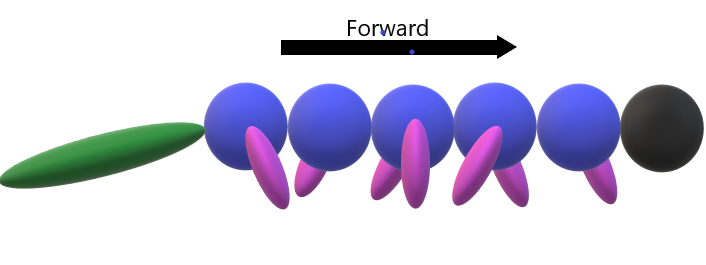
\includegraphics[scale=0.5]{robotDesign}
\caption{An example of a randomly generated robot (viewed from the side).}
\end{figure}


\subsubsection{Body Movement}
The fundamental movement pattern of the body sections will mimic the serpentine motion of a snake, as shown in figure TODO.
\begin{figure}[H]
\centering
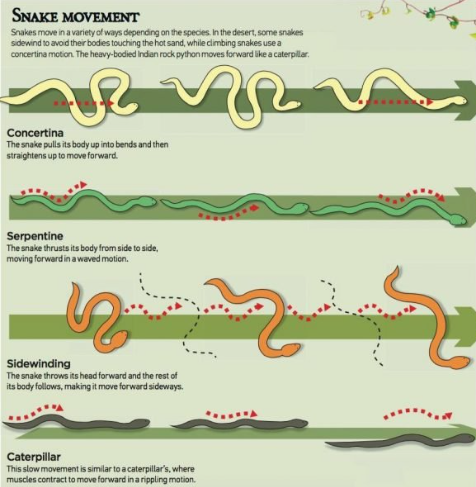
\includegraphics[scale=0.8]{snakeMovement}
\caption{Diagram of different motions snakes use to move. \citep{snakeMovement} }
\end{figure}
\nocitemain{snakeMovement}
To achieve this, each module will have the ability to drive forward and/or rotate and will have its own set of parameters (e.g. speed). To improve the fluidity of the motion a central pattern generator (CPG) approach. A CPG \textit{"can produce rhythmic motor patterns ... in the absence of sensory or descending inputs that carry specific timing information."} \citepmain{cpgDefinition} It is worth noting that the body will not implement a true CPG: the algorithm will utilise a similar approach that avoids any sensory understanding of its worldspace or timing.\\

There will be an option to maintain serpentine motion by alternating the direction of rotation between the rotating sections, and evenly spacing these sections across the body (see figure TODO). The algorithm will not be constrained to this serpentine motion so may move away from this behaviour as it mutates. Nonetheless, due to the embodiment of the robot it is expected that the motion will remain snakelike.\\
\begin{figure}[H]
\centering
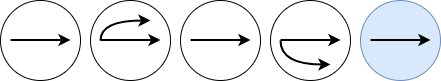
\includegraphics[scale=0.6]{serpentineDiagram}
\caption{The driving \& rotation values used to maintain a serpentine motion.}
\end{figure}

The decision to have the body oscillate as opposed to remaining static whilst the legs provide the entirety of the motion is supported by Jeongryul Kim. Due to a lack of degrees of freedom in legged robots a robot may struggle to maintain its posture and direction of movement. \textit{"A possible solution to such lack of DOFs caused by underactuation may be additional motions of the body"}. \citepmain{bodyOscillation} 
It is important to note that the referenced study was analysing bipedal robots when this conclusion was drawn. To test the assumption that moving the body with the legs improves performance, another experiment will be conducted to explore the impact of the body remaining static. \\
An alternative solution could be to add additional joints for the legs to increase the DOFs. This idea is explored in more detail in TODO. To summarise, whilst considering the positioning of leg joints, a form that mimicked the structure of a lizard was prioritised. The offer of freedom in the leg placement remains as a project limitation. \\
Regardless, other projects have adopted a similar approach with promising results. The Salamandra Robotica II used - and inspired - the combination of leg rotation and body oscillation. \citepmain{salamandra} The Salamandra is covered in more depth later in this report.

\subsubsection{Tail Movement}
The motion of the tail will mirror that of the ‘Agama robot’ whereby the tail flicks up quickly in the opposite direction of the trajectory of the body. \citepmain{agama} The focus of this study was for stabilising a robot as it jumped but it is expected that this counterbalancing of the motion of the body will improve the success of the robot. To test this, an experiment will be performed with and without a tail to determine how it impacts the distance the robot is able to cover. 
\begin{figure}[H]
\centering
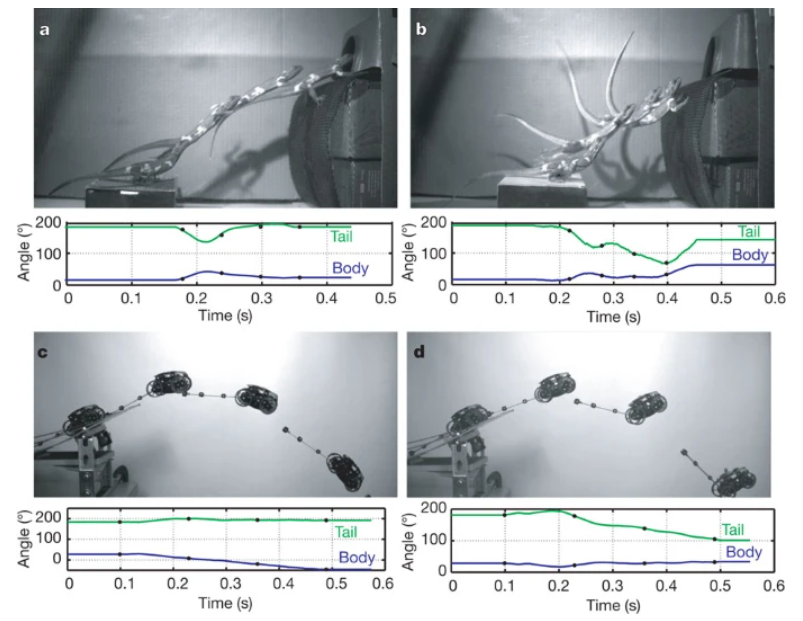
\includegraphics[scale=0.6]{agamaJump}
\caption{An Agama lizard compared to the Agama robot whilst jumping \citep{agama}}
\end{figure}

\subsubsection{Leg Movement}
The approach to the fundamental movement of the legs is inspired by the Salamandra Robotica II. \citepmain{salamandra} Rotating each leg $360^\circ$ in its joint is a simpler mechanism to push the body forward than a biological folding limb. Though the design is somewhat detached from a biological leg, it is hoped that the implementation of a gait will restore a lizardlike motion.\\
To replicate a lizard's gait, diagonally opposite legs will be accelerated in rhythm with the motion of the body. 
\begin{figure}[H]
\begin{minipage}[t]{.4\textwidth}
\centering
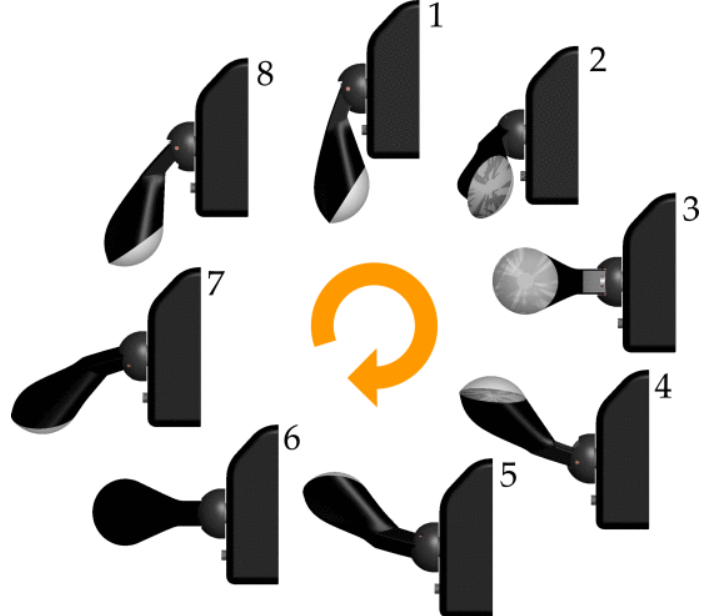
\includegraphics[width=1\textwidth]{salamandraLegSpin}
\caption{The $360^\circ$ leg rotation used by the Salamandra Robotica II \citep{salamandra}}
\end{minipage}
\hfill
\begin{minipage}[t]{.55\textwidth}
\centering
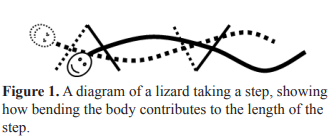
\includegraphics[width=1\textwidth]{lizardGait}
\caption{A representation of the relationship between a lizard's gait and its body oscillation. \citep{reptileLocomotion}}
\end{minipage}
\end{figure}
\nocitemain{reptileLocomotion}

\subsubsection{Genetic Algorithm}
%TODO ADD explanation about why a genetic algorithm was chosen
%TODO ADD research about why the recombination and mutation approach is suited
%TODO ADD explanation about how this approach creates a relationship between the body and movement
%TODO ADD explanation about why I want a relationship between them - article Simon sent
%TODO ADD explain triad recombination - what examples are there of this in nature?
%TODO ADD explain about the red robots - why might these be attractive?
The genetic algorithm aims to optimise the parameters of Lizardbot and, once an optimal robot has been found, could be removed from the project. It has no impact on the behaviour of the robot mid-generation in reaction to specific circumstances.\\

\subsubsection{Dynamic Movement}
\begin{wrapfigure}{r}{0.3\textwidth}
    \centering
    \vspace*{-5mm}
    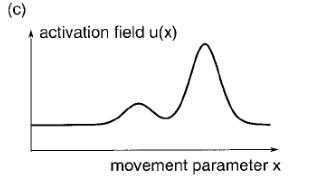
\includegraphics[width=0.3\textwidth]{activationExample}
    \caption{An example of a movement being activated: weakly at first, then again with a stronger activation to produce a greater movement. \citep{dft}}
\end{wrapfigure}
\nocitemain{dft}
Dynamic systems theory uses the causal webs of an environment to determine the \textit{"sequences of states that could take the system from one location in state space to another"}. \citepmain{mindware}
Rather than providing rigid rules about how the robot should move, the robot explores how to move in a direction through trial and error. Essentially, it will 'collect' behaviours. If a specific set of parameters produced a desired behaviour (e.g. move left) then this can be activated with increasing force (see figure TODO) to steer the robot left across the terrain. This approach would produce a behaviour-based approach to navigating the terrain. Thelan and Smith explored the behaviour of babies taking steps on a treadmill and concluded that there was a complex relationship between the body, environment and behaviour. \citepmain{babyStepping} This relationship can be argued as both advantageous for Lizardbot, and a potential constraint to the performance that dynamic movement can offer.\\
The adaptive behaviour can result in emergent complex behaviours that would otherwise have been a mammoth of a task to implement as a set of instructions. On the flipside, dynamic movement relies on assumptions about the relationship between a robot's body, movement, and terrain. It is not feasible to store every factor that culminated in a behaviour and thus the system must be reduced to a select few control parameters. The assumptions that this requires render the dynamic approach unsuitable as the primary movement mechanism. However, it may still complement the movement algorithms discussed in TODO. Andy Clark discusses the idea of "partial programs" \citepmain{partialPrograms} - \textit{"minimal instruction sets that maximally exploit the inherent (bodily and environmental) dynamics of a controlled system"}. \citepmain{mindware} As long as Lizardbot's adaptive behaviour can work alongside other causal influences then dynamic movement is expected to improve its performance.
 




\subsubsection{Terrain Generation}
Three terrains will be generated to test the robot in increasingly difficult environments. The terrains will be randomly generated once and then stored and used as a control variable in experiments.\\ 
The terrain types $[Smooth, Uneven, Rough]$ to be created are inspired by those used to test the Octopus robot \citepmain{octopusRobot}.\\

It is important to consider the situatedness of the Lizardbot. The environment that it is presented with will influence the outcome of its cognition. Specifically, it will influence its situated dynamical cognition. This is defined as “cognition [emerging] from a real-time, continuous and strictly coupled sensorimotor interaction between an unstable subjective experience and an unstable objective world.” \citepmain{situatedness}
It is not feasible to test the interaction between the Lizardbot and every terrain that a robot could encounter. It is, however, possible to expand the terrain to include common properties. It is known that “the friction between the snake robot and the ground, affects significantly its motion” \citepmain{modularDesign}, hence an experiment will be conducted by returning a high-performing group of robots to the terrain with the coefficient of friction adjusted. By varying the texture of surfaces within the environment the Lizardbot may produce different behaviour. \\

Additionally, the smooth terrain will be deliberately featureless to test the behaviour of the robot in a simple environment. Herbert Simon provided an elegant example of the importance of this consideration: an ant is observed making its way back to its nest across a beach.\\
Its route is ‘a sequence of irregular, angular segments’ that suggests some level of complexity in the ant's behaviour. However, the beach for the ant is a much harsher environment than it is for a human. It is more likely that ‘its complexity is really a complexity in the surface of the beach, not a complexity in the ant.’ \citepmain{antsBeach} Thus, the situatedness of the robot could culminate in behaviours that are not of its own making and are instead caused by its relationship with the terrain. The smooth terrain should reduce the role of the environment and allow for emergent behaviours to be prescribed to the robot itself.\\

\subsection{Extension Objectives}
\subsubsection{Vision}
Thus far the Lizardbot has focused on finding the ideal parameters for the overall form and movement of the robot, with additional thought for a dynamic system to allow the robot to react to its situation. There has been little focus on a preemptive approach, which has the potential to reduce the risk of damage to a real robot. When a robot becomes stuck it will likely find itself bouncing against the nearby terrain, forcing the prioritisation of durability in the design of the robot. If the robot were given a rudimentary visual system it could instead anticipate collisions and adjust its course to avoid them.\\
To achieve vision, a camera could be placed in the head of the robot. Unity’s built-in functionality would provide feedback on objects within the range of the camera. This knowledge, when combined with the dynamic systems element of the AI, would allow the robot to make informed ‘decisions’ about how it should approach the terrain it is aware of. \\
This feature would reduce the risk of damage to a physical robot by avoiding collisions with the terrain. David Lee investigated the factors affecting the specific moment in which an agent will begin reacting to an impending collision. He found that for an agent approaching a stationary object, the relative location of the obstacle in the agent’s visual field could be used to deduce the time-to-collision. \citepmain{timeToCollision} The use of this time-to-collision would directly relate to the brief of the project as it applies an algorithm derived from nature to a design problem (in this case collision detection and avoidance). \textit{”Most animals respond avoidantly and directionally to the abstract visual stimulus ... which specifies the approach of an object and impending collision.”} \citepmain{animalCollisionResponse}\\
Implementing a visual system to the Lizardbot could unlock a variety of more complex - \textbf{and proactive} - behaviours.
\subsubsection{Flexible Tail}
%TODO ADD explanation of why a flexible tail would be advantageous

\newpage
\section{Project Relevance}
Lizardbot will incorporate various elements of each of the following projects: from the modular body design to the counterbalancing tail. The modular snake robot had the same goal as this project: to design a robot that could tackle obstacles in rough terrain. Meanwhile the Agama robot was exploring the behaviour of lizards as a stabilisation mechanism.\\
This project will combine the use of a tail for stabilisation, the snakelike motion of the body as the legs move, and the modular design to produce a lizardlike motion. It will not be constrained by the limits of a physical robot, thus evolving the body of the robot in a manner that these example projects were unable to. The AI will add an element of reactivity to a wider array of situations than these robots, as the model will not be seeking a specific behaviour. Rather, it will determine how the behaviour that it is producing influences its success and absorb this knowledge as it navigates the terrain.
\subsection{Modular Snake Robot}
The work of Ye et al. \citepmain{modularRobotBackground} found that a modular snake robot was \textit{“more efficient to get into complicated environments”}. Their aim was to test the abilities of such a robot in environments too harsh for humans. Each module operated independently in a manner similar to the body movement algorithm covered in the project aims. Each module was attached to the adjacent modules via a joint that rotated to create a wave through the body, while a servo drove the module forward. Their robot used a cosine function to manoeuvre the body, whereas the Lizardbot will make use of an approach closer to that of a central pattern generator. \\
The modular snake robot successfully navigated any obstacles with a height less than the height of a module. It also demonstrated the constraints that a physical robot can face (e.g. the error rate in the servos increased with amplitudes over 4cm). Lizardbot aims to explore similar methods of movement to improve \textit{environmental adaptivity}, without the physical limits faced by the modular robot. The addition of legs and a tail to the modular design is intended to enable the robot to overcome more complex obstacles in an environment. Meanwhile the AI will, theoretically, allow the Lizardbot to adapt to its situation more than the modular snake robot was able to.

\subsection{Agama Robot}
The tail-assisted pitch control used to build the Agama lizard-inspired robot will heavily influence the tail motion of the Lizardbot. \citepmain{agama} It will constantly assess the momentum of the robot and adjust the motion of the tail to counterbalance this force. Applying this research may reduce the risk of the robot overbalancing, a situation that could damage a physical robot. The Agama study found that \textit{“the robot with PD feedback tail control maintained a nearly constant body angle by swinging its tail upward and incurred 72\% less rotation after a perturbation than did the robot without tail control”.} This is a promising result for stabilising the Lizardbot.

\subsection{Salamandra Robotica II}
The relevant goal of the Salamandra Robotica II \citepmain{salamandra} was to \textit{“advance robotics design for bimodal and efficient locomotion”}. The design of this robot heavily inspired various elements of the design of the Lizardbot: the full rotation of the legs and the CPG-inspired oscillation of the body. \\
One of the key differences between the Salamandra and the Lizardbot is the method for turning. The former used calculated asymmetric oscillations to produce a curving trajectory (see figure TODO) while the latter will dynamically derive an activation function for a turn. \\
\begin{figure}[H]
\centering
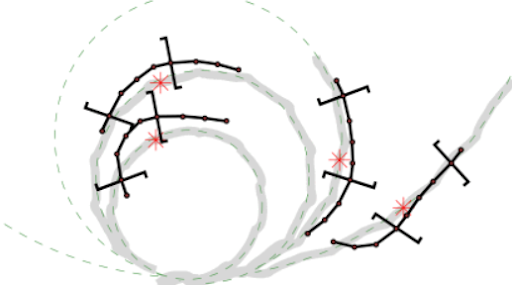
\includegraphics[scale=0.7]{salamandraTurning}
\caption{The results of various curved trajectories of the Salamandra. \citep{salamandra}}
\end{figure}
Another difference was the Salamandra’s passive tail. The tail fin was only used to test its effect on speed whilst swimming; removing it decreased the speed by 63\%. The rigidity of the tail will be matched by this project but, as previously discussed, it will rotate to counterbalance the motion of the rest of the body.

\subsection{tbc}
%TODO Find a team that have modelled a robot vs building one - how about that paper Simon sent

\newpage
\section{Requirements Analysis}
Insert from interim report - needs some work\\
Add section on the constraints of this project

\newpage
\section{Professional and Ethical Considerations}
Insert from interim report with more reference to code of conduct

\newpage
\section{Implementation}
\subsection{Terrain}
Three terrains were generated using Procedural Toolkit \citepsoft{proceduralToolkit} to test the performance of the robot across various environments: rough, uneven, and smooth. 
\begin{figure}[H]
\centering
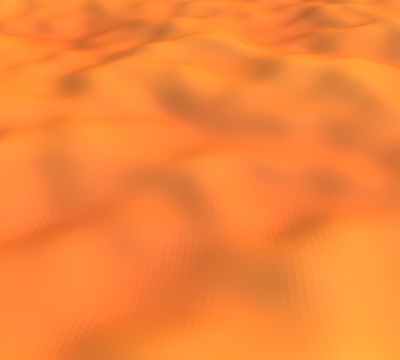
\includegraphics[scale=0.3]{smoothTerrain}
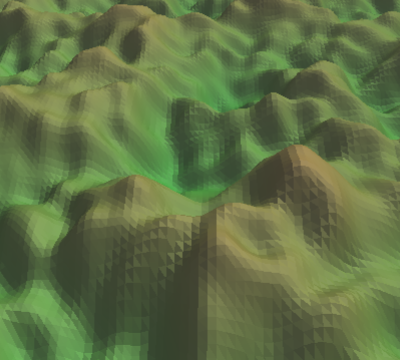
\includegraphics[scale=0.3]{unevenTerrain}
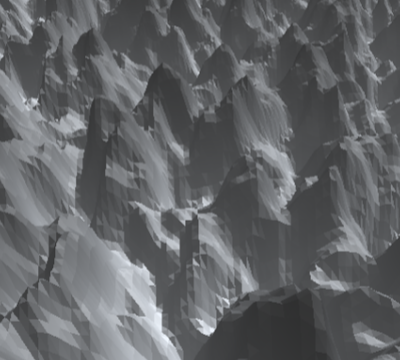
\includegraphics[scale=0.3]{roughTerrain}
\caption{Examples of the three terrain types. (From left to right) Smooth, Uneven, Rough.}
\end{figure}
At one point the height of the terrain was proportional to the number of sections of the robot, a similar method to that of the Octopus robot. However, as the terrain is a control variable the heights were switched to a static value: $Smooth=8, Uneven=16, Rough=24$.\\
Overall, the rougher the terrain, the higher and more closed in it is. Most of the development of the robot was conducted on the smooth and uneven terrains, as the rough terrain aims to provide a more extreme environment with which to test the efficacy of the AI.\\
It is worth noting that the robot is still being tested on three terrains with some common properties (e.g. gravity) and these factors may introduce bias in the AI. This is a reasonable situation as long as applications of the Lizardbot are further modelled on encounterable terrains to allow the AI to adapt the robot accordingly. For proof of concept the sample set of terrains is sufficient.

\subsection{Robot}
\subsubsection{Body}
To create a snakelike body, each body module is attached to the previous module by a configurable joint \citepcode{configJoints} and has two methods of movement: driving and rotation. The physical design of the robot creates a fluid motion before any complex movement is applied. With the joint structure, the movement of one section is translated to those behind it - similar to dragging a piece of string along the ground. This is shown in figure TODO: the head rotates and, after a delay, creates the same angle in the sections behind it.\\
The former applies a forward force as determined by the drive velocity parameter whilst the latter applies a velocity to each module using the following equation:
\begin{center}
\begin{Large}
$\overrightarrow{v_{i}} = \overrightarrow{v_{i-1}} + \frac{m}{2}\overrightarrow{w} $
\end{Large}
\end{center}

For rotating sections $i = 0, ..., m$, where $m \leq n$, the value of $w$ will be calculated using $S$ or $C$ as specified.\\
\begin{center}
\begin{Large}
$S: \overrightarrow{w} = sin\overrightarrow{\theta_{i-1}} + sin\overrightarrow{\theta_{i}}$
\\[1\baselineskip]
$C: \overrightarrow{w} = cos\overrightarrow{\theta_{i-1}} + cos\overrightarrow{\theta_{i}}$\\
\end{Large}
\end{center}
%TODO ADD explanation about rotation multiplier

%TODO ADD comparison with Salamandra Robotica oscillations

This central pattern generator (CPG) approach allows each module to react to the velocity and angle of the previous section. The equation for the CPG originated in Tony Dear’s multi-link snake robot: a robot with a similar modular design with passive joints connecting the modules. \citepmain{cpgRobot} Lizardbot utilises the same math to calculate the velocity with one distinction: Dear’s robot split the velocity vector into its axes, using cos for the x axis and sin for the y. Lizardbot instead calculates the vector as a whole and alternates the rotating sections between sin and cos to produce the serpentine motion. For robots with serpentine motion disabled, $S$ and $C$ will be assigned randomly to the rotating modules.\\

\begin{figure}[H]
\begin{minipage}[t]{.4\textwidth}
\centering
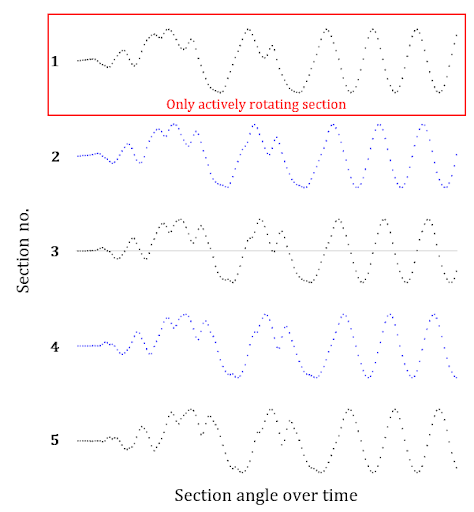
\includegraphics[width=1\textwidth]{cpgMirroring}
\caption{Demonstration of body motion with a single rotating section at the head of the body.}
\end{minipage}
\hfill
\begin{minipage}[t]{.5\textwidth}
\centering
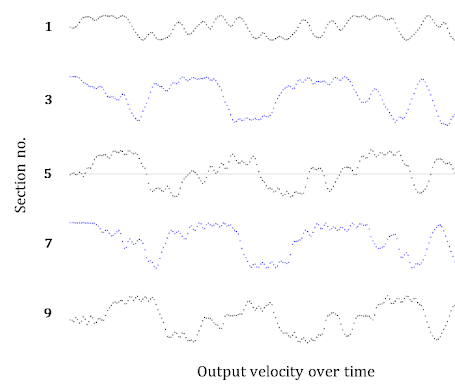
\includegraphics[width=1\textwidth]{cpgSerpentine}
\caption{The output velocities generated by each body module with serpentine motion enabled. Modules using $S$ are shown in black, $C$ in blue.}
\end{minipage}
\end{figure}

As each section ‘reacts’ to the previous one whilst using the opposing equation, the velocity applied is almost an inversion of its predecessor. Moving back through the body there appears to be more fluctuation in the values as more noise is introduced through each application of the equation. The advantage of using this recursive approach is the incredibly organic behaviour that it produces. The first prototypes of the project used hardcoded timings and velocities to try and mimic a serpentine motion and the rigidity of the code was evident in the behaviour. With the above equation applied, the motion of the body appears completely natural. As the Lizardbot slithers through troughs in the terrain or wriggles whilst stuck on a ridge, it is easy to forget that it has no awareness of its surroundings. It is simply reacting to the body that came before it.


\subsubsection{Tail}
The use of a tail has the potential to counterbalance the body and provide stability as the lizardbot moves. The Agama robot used the angular momentum of the body to calculate how to calibrate the tail vertically as the robot jumped. Lizardbot implemented a similar approach in three dimensions by calculating the total momentum of the robot around its centre of gravity (COG) at each frame, and adjusting the velocity of the tail accordingly.\\ 
\begin{figure}[H]
\centering
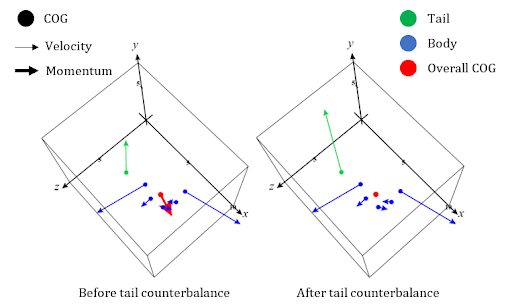
\includegraphics[scale=0.6]{tailMomentum}
\caption{A representation of the tail being adjusted to conserve the angular momentum of a robot. Diagram created using CalcPlot3D \citep{diagrams}}
\end{figure}

For all body parts $i = 0, ..., n$, the radius of the path of motion is the distance from the individual COG $x$ to the COG of the overall robot.
\begin{center}
\begin{Large}
$r = |x_{i} - \frac{1}{n}\sum_{i}^{n}m_{i}x_{i}|$
\end{Large}
\end{center}

The total angular momentum $L$ of the robot is calculated using the above values of $r$, the mass $m$ and the velocity $v$ of each body part. \citepcode{angularMomentum}
\begin{center}
\begin{Large}
$L = \sum^{n}_{i} r_{i}m_{i}v_{i}$
\end{Large}
\end{center}

To conserve momentum, the velocity of the tail is calculated by inverting $L$ and dividing it by the tail's mass and distance from the overall COG.
\begin{center}
\begin{Large}
$v_{t} = - \frac{L}{r_{t}m_{t}}$\\
\end{Large}
\end{center}

Another simplified approach was considered whereby the overall velocity of the robot was counterbalanced instead, however this was found to create sharp changes in the velocity of the tail that could cause it to fling the entire body into the air. Whilst this showed promising behaviour for the basis of a jumping motion, it was counter-productive for a feature whose goal was to stabilise the robot. Additionally, by calculating the magnitude around the COG, any difference in mass between components is taken into consideration. Thus, the tail is able to counterbalance any body structure (assuming that the motion of the tail is not physically blocked by the position of a body part).\\

The design of the tail assumes that nature has already selected for the optimal location by placing the tail at the back of a creature. This assumption seems intuitive. Most animals, including lizards, are symmetrical and the location of the tail maintains this property, alongside keeping the motion of the tail in the same plane as the rest of the body. For Lizardbot, this assumption could be removed in the future. Since symmetry is not a required property for non-uniform bodies, the tail could be placed anywhere that has equal mass either side of the tail - or placed randomly to see what effect this has on the robot. Who am I to say that a tail cannot be located on the head?

\subsubsection{Legs}
Legs were added to Lizardbot in an attempt to match the gait of a lizard.
As inspired by the design of the Salamandra Robotica \citepmain{salamandra}, each leg is designed to rotate in a circle in order to push the body forward. The physical design of the leg matches the elliptical shape of the tail and uses the same configuration of customisable mass and length. 
Currently, there are only two attachment points for a leg on each body module: one each side, perpendicular to the body joints. For a uniform body, the legs are placed symmetrically along the body and given equal length and mass; they are constructed randomly for non-uniform bodies. \\

The leg rotates around an axis perpendicular to the body section it is attached to, as shown in figure TODO. The size of the circle it follows is determined by the angle it is offset by when attached to the body ($\alpha$). \\

\begin{figure}[H]
\centering
$\vcenter{\hbox{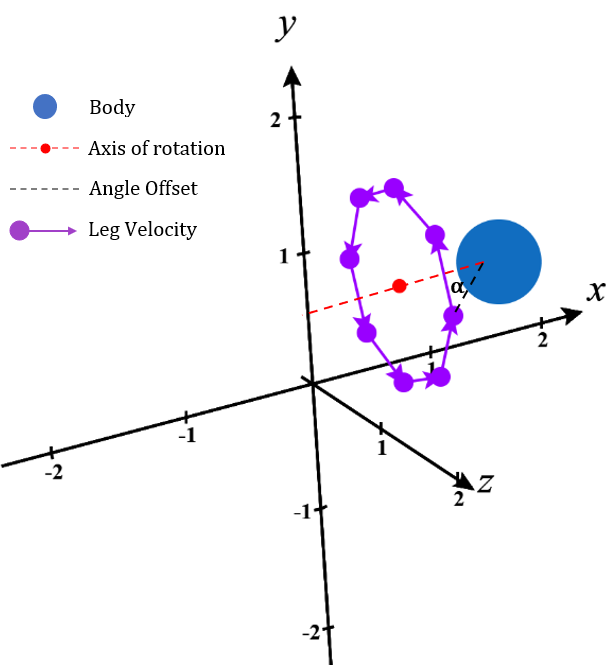
\includegraphics[width=0.5\textwidth]{legCircleDiagram}}}$
$\vcenter{\hbox{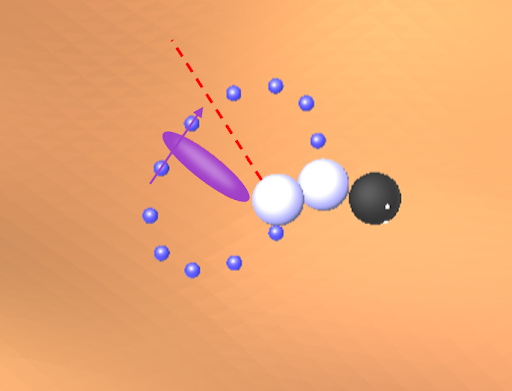
\includegraphics[width=0.4\textwidth]{legCircleExample}}}$
\caption{(Left) An illustration of the rotation of a leg around an axis of rotation. Only one attachment point is shown - another would be available on the other side of the body along the $x$ axis. Diagram created using CalcPlot3D \citep{diagrams}\\
(Right) A leg following its path of motion.}
\end{figure}



The rotation of the leg follows a series of conceptual points spaced $30^\circ$ apart around the point $D$ (shown by the red point along the axis of rotation in figure TODO). These points are generated using the following equation:
\begin{center}
\begin{Large}
$P = D + Vcos\theta + Ucos\theta$\\
\end{Large}
\end{center}

Where $V$ and $U$ are two vectors perpendicular to each other in a plane through $D$ and the target circle, and $0\leq\theta<360$. \citepcode{circlePoints}
 
To calculate the desired velocity of the leg, the point $P_i$ closest to the current position of the leg is found. From this, the new velocity can be calculated using the vector to the next point on the circle.   
\begin{center}
\begin{Large}
$v_{i} = g(P_{i + 1} - P_{i})$
\end{Large}
\end{center}

If the relevant gene is active, the gait multiplier $g$ increases the velocity when the body is turning away from the leg, decreasing it if the body is turning toward the leg.\\

The performance of the legs is analysed in section TODO, though it is presumed that with more work the performance could be drastically improved: currently it resembles a lot of twitching. It is possible that an alternative joint mechanism would allow for Lizardbot to stand on its legs and appear more natural. It would also be interesting to explore how the location of the legs impacts the robot as a whole. Currently the attachment points are based on lizards (indeed, most animals) and the years of evolution that have led to their structure. However, the offer of more variety in the design of the robot may offer alternative solutions to navigate the terrain. 


\subsection{Artifical Intelligence}
A population of Lizardbots can use a genetic algorithm to "evolve" over a series of generations. A genetic algorithm is a form of artificial intelligence that more closely models the characteristics of natural selection. An agent’s parameters are broken down into ‘genes’ that can be manipulated by recombination and/or mutation. The aim of this genetic algorithm (GA) is to improve the performance of the robots over time. The GA is performed when a robot is declared to be stuck by the trapped algorithm. 

\subsubsection{Performance}
The metric used to measure the performance of a robot can heavily influence the outcome of the genetic algorithm. As the desired outcome is a robot capable of navigating the terrain, the base measurement used is the furthest distance (by magnitude) that it has travelled in a given generation from its spawn point within the terrain. 
\\[1\baselineskip]
Two additional parameters are used to add context to this base measurement. 

The first penalises robots that cause large collisions through a body part. Every time a body part encounters a collision it triggers a method that will measure the force that the body part has experienced. Unity's build-in physics system returns the impulse $I$ of a collision. Using this, the force can be found by dividing the impulse by time: {\Large $f = \frac{I}{t}$}. \citepcode{collisionForce}
If the force is found to be above a threshold then the robot will be penalised by deducting 10\% from the performance. \\
This ensures that the robot is not evolving toward a behaviour that carries it across the terrain efficiently but could be damaging to its structure in the physical world. An example of this is an iteration whereby the robots were observed ‘flicking’ their tails rapidly downward, causing the robot to be thrown into the air and across the terrain. Whilst this was effective at getting them to the edge of the terrain within seconds, this approach would shatter most robots upon collision with the terrain. This threshold can be tailored to the needs of the robot, such that robots with shielding or soft-bodies robots can be given a higher threshold to allow more risky behaviour.

The second rewards robots that move quickly. The current performance is multiplied by the average speed (distance / time) of the robot since its spawn. 
\\[1\baselineskip] 
To provide an example of the performance metric, say Robot3 V8 has travelled from (0, 0, 0) to (10, 4, -13) in 21 seconds, and has had two above-threshold collisions. The base performance would be 16.88. Multiplied by its speed, this becomes 13.57. With a 10\% deduction for each collision, the final performance is 10.99. \\
A flaw in this metric is that it does not differentiate between the routes that robots take. If one robot moved quickly but erratically, it may be rewarded equally to one that moved slowly and directly. However, this metric appears to provide a suitable balance between rewarding robots that travel the furthest, further rewarding those that move efficiently, and reducing behaviours that would damage a physical robot. \\

When referring to the performance of a population, the mean performance of the highest performing 25\% is being measured. When a robot is mutated and respawned its performance returns to zero, hence it was found that analysing the entire population added too much noise to the results. 

\subsubsection{Trapped Algorithm}
It is important for the AI to know when the robot is stuck to trigger the termination of the current generation. At this point the AI can mutate the robot before respawning it. This trapped behaviour can take many forms, from bouncing against the same point in the terrain, circling itself, or looping between the same location(s).\\

Initially, the maximum - minimum of the baseline performance metric (magnitude of the distance from the origin) over the last $t$ seconds was used. This approach was heavily flawed as it reduced the data set to a single dimension. \\
Instead, the entire data set over the last $t$ seconds was analysed. The robot was declared stuck when the variance of the robot’s 3D coordinates over $t$ seconds converged to 0. This approach correctly identified the robot as stuck but had one major flaw: travelling in a straight line outputs a variance of 0. This behaviour is highly efficient and, whilst it is not something that the AI will train for, is a behaviour that the AI should absolutely not be training against. These false positives prompted a third approach. \\
The algorithm finds the minimum and maximum values for each axis to draw a conceptual cube around the points the robot has visited in the last $t$ seconds. These cubes depict the  worldspace the robot has recently explored. The variance of the data set is calculated for the volume of the cube rather than the coordinates themselves. If the variance of the volumes of the cubes rounds to zero then the robot is considered to be trapped. \\
\begin{figure}[H]
\centering
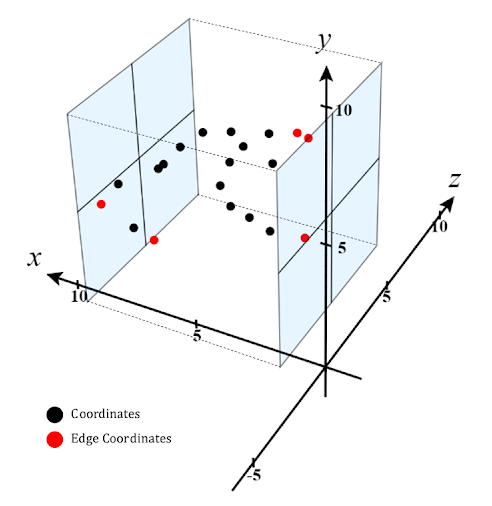
\includegraphics[scale=0.7]{trappedAlgorithm}
\caption{A representation of the cube constructed around the last 20 locations a robot has visited (captured twice a second). Diagram created using CalcPlot3D \citep{diagrams}}
\end{figure}

Finally, the sensitivitiy of the algorithm needed to be determined by adjusting the value of $t$. The results showed that too low a value of $t$ produced false positives due to it not allowing the robot enough time to turn around. In contrast, if $t$ was too high it took longer for the algorithm to identify when the robot was stuck. This would waste time continuing for an extra few seconds each generation, or could potentially miss instances when the robot became trapped but was able to free itself. A sensitivity of $t=20$ appeared to provide a balanced value across all three terrains.

\begin{figure}[H]
\centering
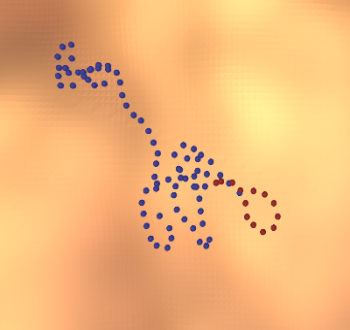
\includegraphics[width=0.2\textwidth]{trappedSmooth}
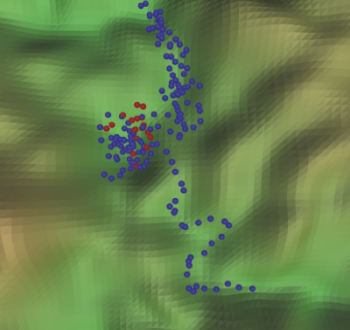
\includegraphics[width=0.2\textwidth]{trappedUneven}
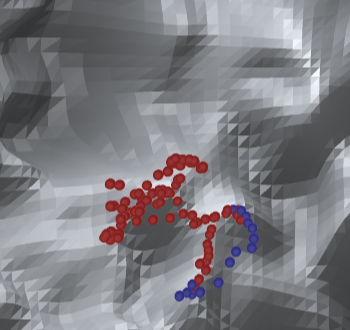
\includegraphics[width=0.2\textwidth]{trappedRough}
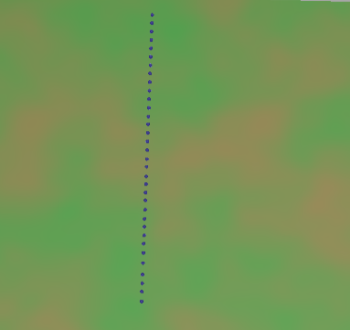
\includegraphics[width=0.2\textwidth]{trappedFlat}
\caption{A demonstration of the trapped algorithm using the same robot and $t=20$ on each terrain.\\
Each blue point represents the location of the robot being captured. Red indicates that the robot is trapped (and would normally have been disabled and passed to the genetic algorithm).\\ 
(From left to right) Smooth, Uneven, Rough, Flat. The latter used a robot with rotation disabled to ensure that a robot travelling in a straight line would not be flagged.}
\end{figure}
The red points in figure TODO align with behaviours that can reasonably be classed as ‘trapped’, however it is important to note that this algorithm was implemented with some bias toward certain behaviours (e.g. looping). For this project, the identification of a trapped robot appears sufficient and is expected to produce an AI that will train away from continually exploring the same area for too long. The algorithm has other potential applications in finding looping patterns in any problem that can be assigned a world space. For example, a neural network could be analysed with this algorithm to determine when it is ‘stuck’ whilst performing a task, or a search algorithm could implement it to avoid excessively exploring within a section of the graph. 


\subsubsection{Genes}
The manipulatable characteristics of a robot are distinguished by a \textit{Gene} class. Each variable is instantiated with a default, minimum, and maximum value. Additionally, they are given a type (established in the enum class \textit{Variable} whereby negative enum values are physical properties and positive are movement) to ensure that the recombination covered in section TODO is combining the same genes with each other. \\
This class handles any erroneous situations that arise and allows boolean values to be stored as a float. If the \textit{Get} method of a boolean \textit{Gene} is called, then true will be returned for values greater than 0.5. This allows boolean genes to be mutated slowly (e.g. from 0.35 to 0.6) without having to make a single toggle from one value to the other. \\
When a gene is mutated, if the new value lies outside the valid range then it is 'bounced' (e.g. $max=0.5, v\rightarrow0.6 \Rightarrow v=0.4$). If a value outside the max/min values is passed directly then the max/min value would be assigned instead.

\subsubsection{Population}
To avoid interaction between robots, the body parts of a robot should be capable of colliding between themselves and the terrain but should ignore those of other robots. In Unity, this can be achieved by placing all robot objects into a layer. \citepcode{layerMethod} You can then change the Physics system to ignore collisions between different robot layers.\\ 
Unity’s layers have a limit of 25 available layers. At first, a script was added to every robot scanning around it for other robots in the same layer. Upon detection, the current robot would be moved to another layer that no robots in the vicinity were using. Given that every robot spawned in the same location this script absolutely throttled the performance of the program. With a population of 50 the frame rate would drop from ~200fps to ~20fps. This is not an acceptable impact so an alternative approach was considered. Multiple terrains are generated and 25 robots placed into each. This has the added benefit of being able to generate a population of robots being tested on all three terrain types simultaneously. 


\subsubsection{Genetic Algorithm}
When the trapped algorithm determines that a robot is stuck it is disabled and passed to the genetic algorithm (GA).\\
\begin{figure}[H]
\centering
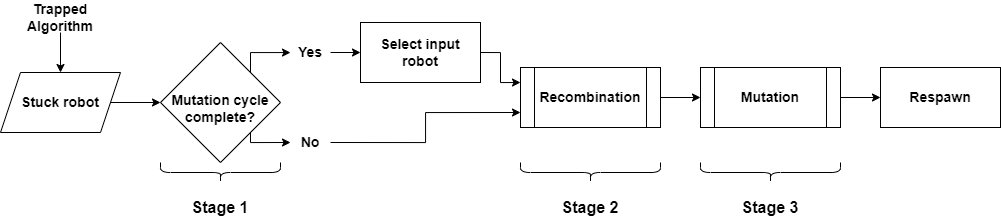
\includegraphics[scale=0.4]{gaProcess}
\caption{The process the genetic algorithm will follow. Diagram created using draw.io \citep{drawio}}
\end{figure}
The GA first selects which robot should be used as the input for the rest of the process. The default input is the stuck robot, however when a mutatio cycle has been completed this may be overruled. The mutation cycle, exemplified in figure TODO, of a robot refers to how many evolutions should take place before the resultant robot is compared to the robot it initially branched from. When a mutation cycle is complete, the highest performing of the two is selected as the input for the GA. The reasoning behind this is to allow a robot to mutate to a lower performing robot temporarily, as this may allow it to evolve into a more successful robot a few generations later. If the mutation cycle is set to 1 then any single evolution that reduces the performance will be rejected.\\
\begin{figure}[H]
\centering
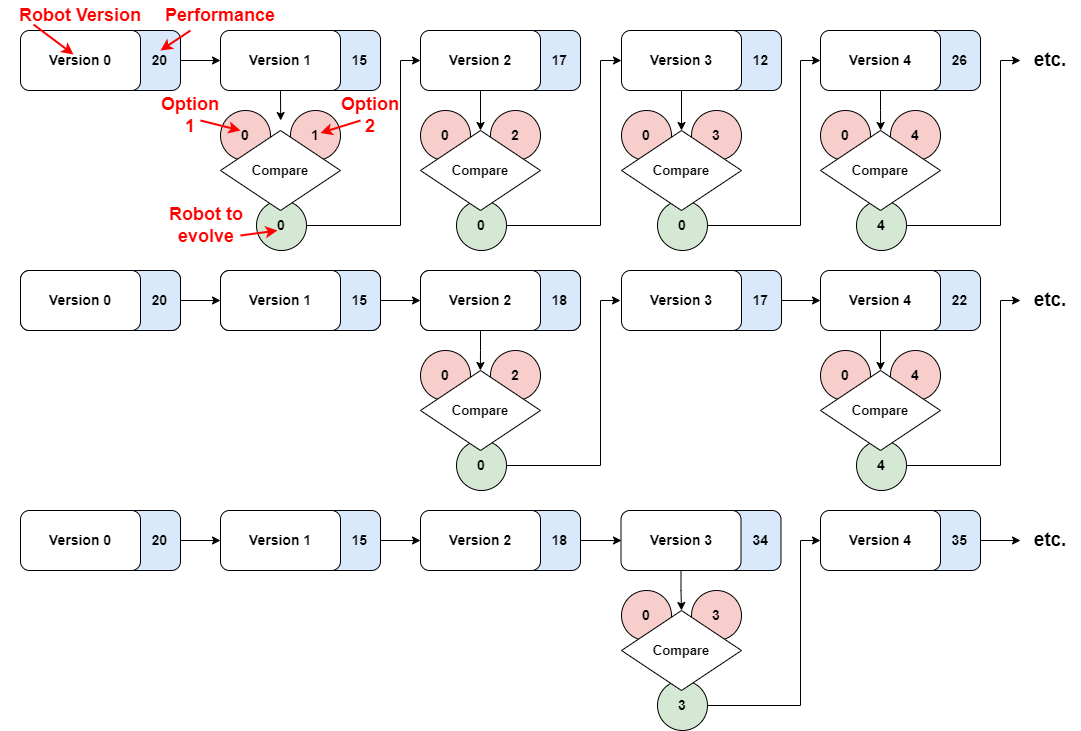
\includegraphics[scale=0.4]{mutationCycle}
\caption{Examples of potential evolutions of a robot. From the top row downwards, the mutation cycle is set to 1, 2, and 3 respectively. Diagram created using draw.io \citep{drawio}}
\end{figure}

Once the input robot has been determined, this robot is then recombined. There are several methods of recombination available but the overall process is: select $k$ robots using a given method and "breed" the genes of one robot in this pool with those of the input robot.\\
The available recombination methods are:
\begin{enumerate}
  \item Physical\\
The selection pool consists of robots that are physically similar to the input robot. The acceptable margin of difference is increased until k robots are found. This method aims to return robots from the population that have a similar number of each body part, and are matching the input robot as to whether to maintain a uniform body.  bullet.
  \item Movement\\
The selection pool consists of robots that are moving in a similar way to that of the input robot. As above, the acceptable margin of difference is incrementally widened if necessary. The selected robots will be following the same rules for maintaining serpentine motion and the gait of the legs. Additionally, they will have a similar ratio of drive velocity to the number of sections to provide an overview for how powerful the robot is. It allows for differences in the rotation of the body as it is hard to implement a sufficient comparison between them. 
	\item Triad\\
This approach is more artificial than others. Two robots are selected: one each from the physical and movement methods. The genes of these two robots are then recombined with the input robot. As discussed in section TODO, nature does demonstrate examples of more than two agents mating.
	\item Lizard\\
This method aims to mimic a more lizardlike breeding process. A characteristic with no direct bearing on the performance is used to select robots that are nearby the input robot, ignoring those in the population on the other side of the terrain. \textit{Nearby} is relative to the spawn point of the robot, and limited to those in the same terrain type. \\
The colour of the body was chosen as the desirable trait; Lizardbot loves blue.\\
In theory, this method should create local ‘ecosystems’ in the population over time as robots that explore the same area of the terrain each iteration will always interact with the same selection pool. 
	\item Random\\
A random robot is selected from the population, to act as a control method.
	\item Any\\
Methods 1-4 make an assumption that using the same method for every generation is optimal. This method instead randomly selects one of the above methods for a single generation.
\end{enumerate}
Each of the input robot's $n$ genes is recombined as follows:
\begin{center}
\begin{Large}
$G(1)_{i} = R^{[0, 1]} < r \longrightarrow$ 
\begin{LARGE}
$^{R^{[0, 1]} < 0.5\longrightarrow G(1)_{i}} 
_{R^{[0, 1]} \geq 0.5 \longrightarrow G(2)_{i}}$
\end{LARGE}
\end{Large}
\end{center}

Where $i = 0, ..., n$. R denotes a randomly generated number in the range $[a, b]$. G(1) refers to the input robot, whilst G(2) is the selected robot. For \textit{Triad} recombination G(2) is randomly chosen from either of the two selected robots, with equal probability.
\\[1\baselineskip]
The recombined robot is then mutated. The genes are divided into physical or movement properties to allow the mutation to be limited to one or the other, or both. As with the recombination, there is also the option for Any mutation, whereby one of the three options is randomly selected every generation. 
The mutation rate, m, is used to avoid mutating every single gene.\\
When a gene is mutated its value is adjusted as follows:
\begin{center}
\begin{Large}
$G_{i} = R^{[0, 1]} < m \longrightarrow $
$(max(G_{i}) - min(G_{i})) R^{[0.01, 0.1]}  G_{i}$\\[1\baselineskip]
\end{Large}
\end{center}
The GA contains four major parameters that influence its function: recombination rate, mutation rate, selection size, and mutation cycle. To determine the optimal values for these, 47 iterations were run with randomly generated values and the performance of the population measured. Each iteration contained 50 robots running for 600 seconds.
The desired outcome was a performance curve that sloped upwards over time. Peaks and troughs were expected as the successful robots returned to the spawn point; the overall pattern of the performance was key. 
\begin{figure}[H]
\centering
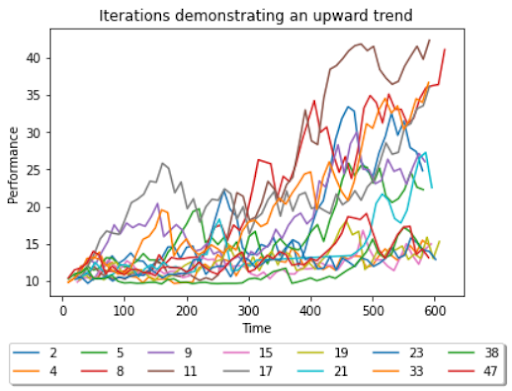
\includegraphics[width=0.45\textwidth]{gaPatternIterations}
\includegraphics[width=0.45\textwidth]{gafilteredIterations}
\caption{(Left) All iterations demonstrating a promising upward trend.\\
(Right) Iterations from the left graph filtered to those that reached a performance $>20$.\\
Graphs created using Colab, \citep{colab} Pandas, \citep{pd} MatPlotLib, \citep{plt} NumPy. \citep{np}}
\end{figure}

Upon analysing the four values being used for the highest performing upward-trending iterations it appeared that successful values had been found through an issue in the code. When generating random values, Unity cycles through the same values if not provided with a seed. \citepcode{randomRepeating} As the four values were consistently the first four values generated they had been repeatedly set as $[2, 0.77, 0.31, 9]$. Of the 8 iterations that showed an upwards trend and performed well, 7 were these values. Additionally, there was only a single iteration using these values that did not perform well. Given the apparent success of these GA values, these were selected as the default parameters. \\
It would be useful to have different GA parameter values tailored to each combination of the recombination and mutation methods. Currently, effective values have been found whilst the Any option was selected for both in an attempt to find parameters suitable for all permutations. However, this may favour certain combinations more than others and there is currently no data on this. Rather, these base values are assumed to be appropriate and the effectiveness of the methods themselves judged relative to them. Ideally, there would be a set of values for each combination, or the ability for the GA parameters to themselves be mutated. \\

There is an assumption that asynchronous evolution is superior to synchronous evolution. The alternative would be to allow every robot to operate for $x$ seconds before mutating a percentage of the population in parallel. This would ensure that every robot experiences the same number of generations and remove any assumptions in the algorithm used to declare a robot as trapped. \\
Intuitively, the current approach is more appropriate as it does not leave unsuccessful robots continuing past the point where they have been identified as trapped. It is also more natural: we do not wait for a person’s 30th birthday before allowing them to have children based on how successful they have been thus far in their lives. Certainly it is more efficient, as waiting for every robot to be declared stuck before mutating a portion of the population would be extremely time consuming. However, it would be useful to gather results of the alternative approach to support this intuition. \\

\subsection{Dynamic Movement}
As outlined in TODO, a dynamic approach uses the historical movement of the robot to ‘learn’ how to move in a given direction again. 
Take a robot that moves left by rolling over. Due to the reactive nature of the algorithms used for movement, it can be assumed that applying the same velocities from the start of the roll would produce another leftward motion. The dynamic movement algorithm saves these velocities for use when a robot needs to move left again. \\
\begin{wrapfigure}[14]{r}{0.25\textwidth}
    \centering
    \vspace*{-5mm}
    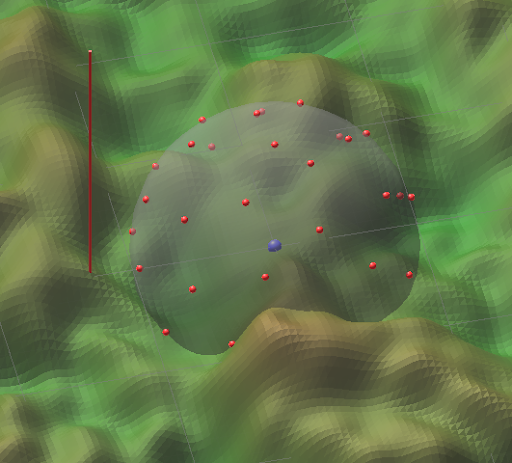
\includegraphics[width=0.25\textwidth]{spherePoints}
    \vspace*{-7mm}
    \caption{A sphere created using a Fibonacci lattice ($n=50$) around a centre point shown in blue.}
\end{wrapfigure}
To achieve this, the worldspace around a robot is divided. \textit{“The Fibonacci lattice is a simple way to very evenly distribute points [on the] surface of a sphere”}. \citepmain{fibonacci} Using the implementation of the Fibonacci sphere provided by Fnord, \citepcode{spherePoints} a series of $n$ points were constructed in a sphere around the robot. It was necessary to strike a balance between too low a value of $n$ producing inaccurate results, which could cause the robot to veer off to one side of the intended direction. Meanwhile, too high a value of $n$ would be unnecessarily expensive and result in the majority of the points containing $null$ values. $n=50$ was selected as an appropriate granularity.\\

The sphere points are relative to the centre of the sphere, thus acting as vectors in the direction of the point. To track how the robot moved in a direction, every $t$ seconds the velocities of each body part are stored. A conceptual sphere is constructed around the initial position of the robot and rotated to match the rotation of the robot. This way, a point directly to the left of the robot rotated $30°$ around an axis will be in the same relative location to the robot at $120°$. \\
Given another interval of $t$, a vector is calculated from the initial position to the resultant position. The sphere point closest to this vector is found by comparing the angle between the vector and the points. 
If there are already values stored for this point then the set of values that moved the robot the furthest distance in the time interval are saved. This process of saving the velocities used to move toward a point is illustrated in figure TODO. 
\begin{figure}[H]
\begin{minipage}[t]{0.3\textwidth}
\centering
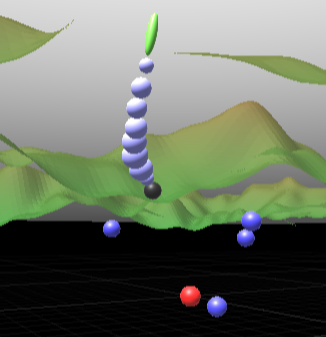
\includegraphics[width=1\textwidth]{storingVelocities}
\vspace*{-7mm}
\caption{Each blue point represents a set of stored velocities for a robot that moved left before turning right and moving downward.}
\end{minipage}
\hfill
\begin{minipage}[t]{0.65\textwidth}
\centering
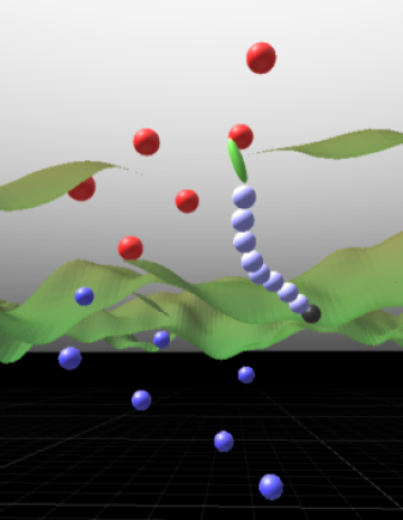
\includegraphics[width=0.4\textwidth]{dstFiltered}
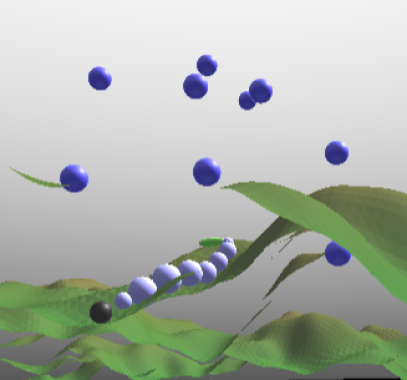
\includegraphics[width=0.55\textwidth]{dstFilteredMissing}
\vspace*{-3mm}
\caption{(Left) A wedge of points that would take the robot away from its spawn point. Those shown in red are those remaining after filtering for the height of the terrain.\\
(Right) An example of the terrain height filtering missing a point.} 
\end{minipage}
\end{figure}

\noindent There are two situations in which the motion of the robot is adjusted:
\begin{enumerate}
\item Routine adjustment\\
The goal of this adjustment is to keep the robot moving away from its spawn point. Every $x$ seconds the vector between the spawn point and the current position of the robot is calculated. The sphere around the robot is filtered using this vector to output a vertical wedge of points moving away from the origin. Applying any of the velocities saved at these points would theoretically direct the robot further across the terrain. \\
The points are further filtered by removing those that have not had any velocities stored yet and those that would move the robot below the level of the terrain. Due to the varying height of the terrain, three measurements are taken at incremental distances from the robot. If the direction of the point at this distance would take it below the height of the terrain then it is removed from the selection. This method aims to take a snapshot of the rough height in a given direction and is liable to miss points that should be eliminated if the peak is between the snapshots. \\
From the filtered points, a single one is selected and the velocities applied to the robot. \\
Frequent adjustment may affect the ability of the robots to explore new means of movement. To reduce this, the regular adjustment is only enacted if the robot is not already moving toward any of the points in the initial wedge. 
\item Scaled adjustment\\
This adjustment is used when the robot is found to be stuck by the trapped algorithm.\\
At this point it is worth mentioning how the activation of the velocities is implemented. For the routine adjustment the applied velocities will be multiplied by a static activation rate. When a robot is trapped, this activation function is increased exponentially in an attempt to free the robot. Failing that, it is mutated and respawned. 
\begin{figure}[H]
\centering
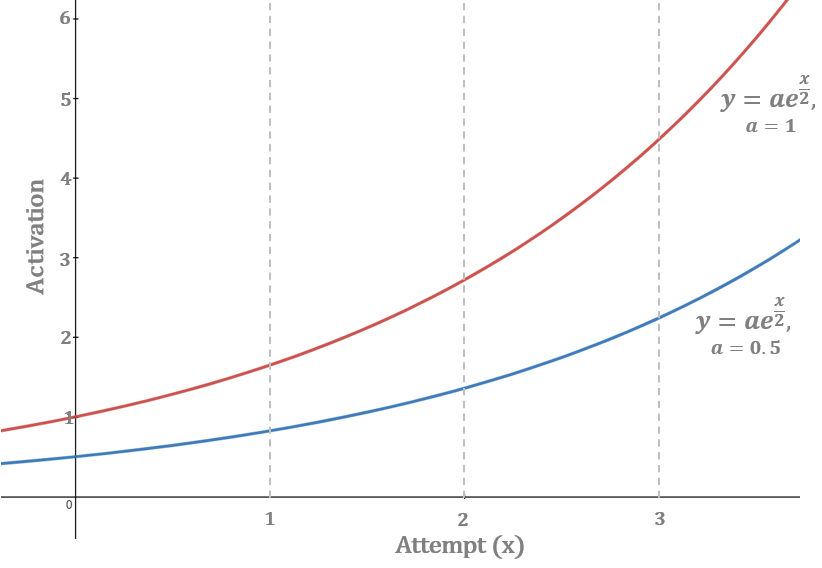
\includegraphics[scale=0.8]{activationFunction}
\caption{The activation multiplier used for each attempt at scaled adjustment. The static activation rate is shown as $\alpha$. Graph created using Desmos. \citep{graphs}}
\end{figure}
\end{enumerate}

It is expected that the dynamic movement algorithm will favour robots that are already performing well. All stored velocities are cleared when the robot is mutated, thus the robots will begin “learning” from scratch every time they become trapped. For robots with sufficient data about their movement, the scaled activation will theoretically enable them to progress in the terrain more often, thus reducing the mutation frequency. As they spend longer in the terrain, less successful robots will have longer to recombine with them. It is predicted that the dynamic movement will both improve the performance of any individual robot, and increase the rate of improvement across a population. \\

\subsection{UI}
A basic UI was added to make it easier to follow the progress of a robot. Whilst the UI itself adds little to the project and the values shown are not particularly self-explanatory, it did uncover a series of bugs in the code that otherwise would have gone unnoticed until the final data collection. It also provided some visibility as to what the code is doing as it mutates the robot, and to the performance of a given robot.\\
It offers two options: \textit{Overview} to watch the population from above, or \textit{Robot} to follow a specified robot. Expanding the \textit{Robot} view reveals a rough view of the values being used. Due to the amount of data being shown without much explanation, it is more of a debugging tool than it is a polished UI. For its purpose it has proven extremely useful. 
\begin{figure}[H]
\centering
\centerline{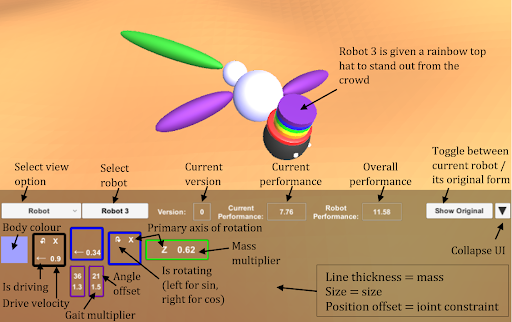
\includegraphics[scale=0.8]{ui} }
\caption{An example of the \textit{Robot} UI view, and an explanation of what each value represents. }
\end{figure}
The UI could be extended to offer a better UX and to offer a view of the performance at runtime. The introduction of a settings page would enable a user to provide constraints for the robots being generated and for the genetic algorithm itself. Currently these constraints can be provided within the various \textit{Config} classes, but a customised menu would lower the threshold to the project as the user would no longer require Unity experience to interact with it. 

\newpage
\section{Results}

\subsection{Evolved Lizardbot}
%TODO when left to it - what do the eventual robots look like? What is the corresponding behaviour?

\subsection{Recombination Methods}
%what impact do the various methods have on performance?

\subsection{Oscillating vs Static Body}
%TODO what happens when the body rotation is turned off?

\subsection{Serpentine Motion}
%TODO what happens when the serpentine motion is fixed to on/off?

\subsection{Counterbalancing Tail}
%TODO does removing the tail help?

\subsection{Leg Gait}
%TODO does removing the legs help? How does the lizard gait impact performance?

\subsection{Uniform vs Non-uniform Robot}
%TODO what happens when uniform body is fixed to on/off?

\subsection{Dynamic Movement}
%TODO what impact does the dynamic movement have on the performance?

\subsection{Terrain Friction}
%TODO what happens to the performance when the same robots are placed on terrains with different frictions?

\subsection{Physical vs Movement Evolution}
%TODO what happens when the mutation & recombination are limited to either physical or movement, or both


%GA report
Whilst the GA demonstrates promising results, there are still some fundamental issues with it. A major issue is that not all genes have equal weight. If the gene that determines whether a uniform body is maintained mutates from false to true then this has a significant effect on the robot. The physical properties of almost all body and leg parts will be adjusted, resulting in a much larger adjustment to the robot than those caused by mutating other genes. To mitigate this, it would be useful to apply weights to each gene. Thus, the mutation range could be scaled accordingly, or the genes categorised such that a change to a heavily weighted gene would limit any changes to other genes. This would allow an isolated analysis of the effect that such a large mutation has on the performance.\\


TODO anecdotal evidence of complex behaviour emerging\\


%DST report
The dynamic movement could be further improved by performing a more comprehensive analysis of the entire terrain around the robot and making a more informed decision about the direction the robot should move in. This could further prevent the robot from becoming trapped as it avoids higher ground or uses a larger activation to “jump” onto higher ground.\\ Additionally, the algorithm currently makes assumptions about the knowledge the robot has about the world around it. It is assumed that there are sensors capable of detecting the rotation, relative position from the origin, velocities of each body part, and of detecting the height of the terrain. It is not immediately obvious how to offer this functionality without the use of these measurements but an exploration into alternative methods may be valuable if the program were to be applied to a physical robot. \\
%TODO add explanation here from mindware about how perception is irrelevant - the outcome is more important. Relationship between \theta and v


%Vision extension report
Adding a rudimentary vision system would enable the AI to make decisions, as opposed to using the successor function to learn entirely from hindsight. By analysing its surroundings it could preemptively determine which route would have the highest odds of success from previous experience. I anticipate that this feedback loop would drastically increase the distance that the model achieves. 



\newpage
\section{Conclusion}

\newpage

\section{References}
\nocitesoft{*}
\nocitecode{*}

\bibliographymain{References/References}
\bibliographysoft{References/SoftReferences}
\bibliographycode{References/CodeReferences}
\newpage
\section{Appendices}
\subsection{Progress Logs}
%TODO add progress logs links
\subsection{Code of Conduct}
%TODO add code of conduct
\subsection{Project Proposal}
%TODO add project proposal



\end{document}